\documentclass[conference]{IEEEtran}
\usepackage[T1]{fontenc}
\usepackage{cite}
\usepackage{amsmath}
\usepackage{booktabs}
\usepackage{array}
\usepackage{graphicx}
\usepackage{url}
\usepackage[hidelinks]{hyperref}
\usepackage{xcolor}
\usepackage{float}
\newcommand{\todo}[1]{\textcolor{red}{[#1]}}

\begin{document}
\sloppy

\title{How Robust Are Exception Handling Defect Models?\\
A3: Preliminary Evidence Report}

\author{\IEEEauthorblockN{Group 9: Emmanuel Adegboye, Benjamin Emeshili, Marco Spensieri}
\IEEEauthorblockA{Software Maintenance and Evolution, Ontario Tech University\\
Artifacts: \url{https://github.com/Detola12/software_replication}}}

\maketitle

\begin{abstract}
We report preliminary evidence for our replication of de P\'adua and Shang (MSR 2018). After fixing a one-line bug in the authors' package, we reproduce every row of the paper's Table 4 and every exception handling metric in its Table 5, on two operating systems. We then varied five modeling settings one at a time. Of the 15 exception handling findings in the reproduced models, 3 hold in all nine configurations and 12 hold in five to eight; none is fragile. Anti-patterns add explanatory power over the base model in 24 of 27 project-configuration pairs (the other three are within seed noise), while the paper's conclusion that flow metrics add nothing for Umbraco reverses under four of the eight changed configurations.

\end{abstract}

\section{Research Questions and Progress}
We replicate de P\'adua and Shang~\cite{padua2018msr}, who modelled whether a source file has a post-release defect using traditional metrics (BASE), BASE plus exception flow characteristics (BSFC), and BASE plus 17 exception handling anti-patterns (BSAP), on Hadoop, Hibernate and Umbraco. Prior work shows that modeling choices such as how correlated metrics are removed can change which metrics a defect model calls important~\cite{jiarpakdee2021tse,shepperd2014bias}, so we test the original findings under changed settings. Our questions are unchanged since Milestone~2:
\begin{itemize}
\item \textbf{RQ1 (Reproducibility):} Does the published package reproduce Tables 4 and 5 of the paper? \emph{Answered in Section~\ref{sec:repro}.}
\item \textbf{RQ2 (Sensitivity):} Do the significant exception handling metrics stay significant, with the same sign, when one modeling setting changes at a time? \emph{Preliminary answer in Section~\ref{sec:sens}, Table~\ref{tab:stab}.}
\item \textbf{RQ3 (Robustness of the conclusion):} Does the gain in explanatory power of BSAP and BSFC over BASE survive those changes? \emph{Preliminary answer in Section~\ref{sec:sens}, Fig.~\ref{fig:gain}.}
\end{itemize}

\textbf{Changes since Milestone 2.} Three changes, each driven by evidence. (1) We fixed the BSFC bug reported in A2 and verified the corrected model against the paper, so RQ2 and RQ3 now cover all three models instead of only BASE and BSAP. (2) We added a second, concept-level stability check (Section~\ref{sec:methods}) because a lower correlation cutoff can swap an anti-pattern's ``total'' metric for its ``average'' twin; counting only exact metric names would mislabel such a finding as fragile. (3) All runs now execute on Linux with a fixed seed, which separates real sensitivity from bootstrap noise. The scope (three projects, five settings, one setting at a time) is unchanged.

\section{Methods Executed}\label{sec:methods}
\textbf{Data.} The authors' replication package, unchanged (SHA-256 prefixes \texttt{2d6387a9} for the scripts and inputs, \texttt{6a8eee1f} for the merged dataset). The models use files with at least one catch block: 890 (Hadoop), 440 (Hibernate) and 230 (Umbraco).

\textbf{Environment.} Ubuntu 24.04, R 4.3.3, rms 6.7.1, Hmisc 5.1.1, caret 6.0.94, e1071 1.7.14. Our A2 baseline was run on Windows 11 with R 4.6.1, so the reproduction now covers two operating systems and two R versions.

\textbf{Procedure.} We made the authors' helper functions read five settings from a configuration file instead of hard-coded values: the correlation cutoff, the files-per-predictor budget, the redundancy cutoff passed to \texttt{redun()}, whether the $\log_{10}(x+1)$ transform is applied, and the significance threshold used both by backward selection (\texttt{fastbw}) and by the Wald tests. Each change is marked \texttt{\# CHANGED} or \texttt{\# FIX} in the code. A runner script executes Section~2 of the authors' model notebook (the files-with-catch-blocks models behind Tables 4 and 5) once per configuration, with \texttt{set.seed(2026)} and the original 1,000 bootstrap repetitions of the optimism-reduced bootstrap~\cite{tantithamthavorn2017tse}. The budget of one predictor per 15 files follows Harrell~\cite{harrell2015rms}, so we test 10 and 20 around it. We ran ten configurations (Table~\ref{tab:configs}). The data preparation notebook was run once and its output reused.

\begin{table}[!h]
\centering
\caption{Configurations executed (one setting changed at a time)}
\label{tab:configs}
\footnotesize
\setlength{\tabcolsep}{4pt}
\begin{tabular}{@{}lll@{}}
\toprule
Configuration & Setting changed & Value (orig.) \\
\midrule
original\_bug & none (published code) & \\
original & BSFC fix (kept in all below) & \\
corr\_0.6 / corr\_0.8 & correlation cutoff & 0.6 / 0.8 (0.7) \\
budget\_10 / budget\_20 & files per predictor & 10 / 20 (15) \\
redun\_0.8 & redundancy cutoff $R^2$ & 0.8 (0.9) \\
no\_log & transform & none ($\log_{10}(x+1)$) \\
p\_0.01 / p\_0.10 & significance threshold & 0.01 / 0.10 (0.05) \\
\bottomrule
\end{tabular}
\end{table}

\textbf{Measures.} For RQ1 we compare the predictor budget, number of potential predictors, adjusted correlation cutoff, optimism-reduced Nagelkerke $R^2$ and significant metrics with Tables 4 and 5. For RQ2, each exception handling metric that is significant in the \emph{original} configuration gets two scores over the nine fixed-code configurations: \emph{exact} (the same metric is significant with the same sign) and \emph{concept} (the same metric or its average/total variant, for example \texttt{Sum.of.AP.Dummy.Handler} and \texttt{Avg..AP.Dummy.Handler}). Following our proposal, a finding is \emph{robust} at 9/9, \emph{moderately robust} at 5--8, and \emph{fragile} at 4 or fewer. For RQ3 we compute the gain in optimism-reduced $R^2$ of BSAP and BSFC over BASE in each configuration.

\textbf{New issue found while running.} All five input CSVs start with a UTF-8 byte-order mark. Under a non-UTF-8 locale (the default ``C'' locale on many Linux servers), R reads the first column name with the mark attached and the merge in the data preparation notebook stops with ``\texttt{'by' must specify a uniquely valid column}''. Setting \texttt{LANG=C.UTF-8} fixes it without code changes; the README now says so.

\section{Preliminary Findings}
\subsection{Reproduction of the original study (RQ1)}\label{sec:repro}
Table~\ref{tab:repro} compares the paper's Table 4 with the authors' code as published and with our one-line fix. The published code reproduces BASE and BSAP exactly but builds BSFC from the BSAP data (A2). With line 223 of \texttt{construction\_functions.R} disabled, BSFC reproduces too: the number of potential predictors (31, 27, 23), Umbraco's forced correlation cutoff of 0.24, and the optimism-reduced $R^2$ all match. Umbraco BSFC is 0.08 against the paper's 0.09; across five seeds it ranges from 0.085 to 0.093, so the gap is bootstrap noise. The fix was first made and run independently by a group member on Windows with R 4.6.1 (pull request \#1, \texttt{output/bsfc\_fix\_run/}). That run selects identical models and significant metrics, and its optimism-reduced $R^2$ values are within 0.008 of ours (Umbraco BSFC 0.093).

\begin{table}[!h]
\centering
\caption{Paper (Table 4) vs.\ published code vs.\ fixed code}
\label{tab:repro}
\footnotesize
\setlength{\tabcolsep}{2.6pt}
\begin{tabular}{@{}llccc@{}}
\toprule
 & & Pot.\ predictors & Corr.\ cutoff & Opt.-red.\ $R^2$ \\
Project & Model & paper/pub./fixed & paper/pub./fixed & paper/pub./fixed \\
\midrule
Hadoop & BASE & 10 / 10 / 10 & .70 / .70 / .70 & .33 / .33 / .33 \\
 & BSAP & 23 / 23 / 23 & .70 / .70 / .70 & .35 / .35 / .35 \\
 & BSFC & 31 / \textbf{23} / 31 & .70 / .70 / .70 & .37 / \textbf{.35} / .37 \\
\midrule
Hibernate & BASE & 18 / 18 / 18 & .70 / .70 / .70 & .21 / .21 / .21 \\
 & BSAP & 19 / 19 / 19 & .70 / .70 / .70 & .23 / .23 / .23 \\
 & BSFC & 27 / \textbf{19} / 27 & .70 / .70 / .70 & .28 / \textbf{.23} / .28 \\
\midrule
Umbraco & BASE & 12 / 12 / 12 & .70 / .70 / .70 & .09 / .09 / .09 \\
 & BSAP & 16 / 16 / 16 & .67 / .67 / .67 & .18 / .18 / .18 \\
 & BSFC & 23 / \textbf{16} / 23 & .24 / \textbf{.67} / .24 & .09 / \textbf{.18} / .08 \\
\bottomrule
\end{tabular}\\[2pt]
\raggedright\scriptsize Budgets (59, 29, 15) match for all nine models. Bold: differs from the paper. Fixed-code values from the \texttt{original} configuration, seed 2026.
\end{table}

The significant metrics also match Table 5. With the fix, BSFC selects exactly the paper's flow metrics: for Hadoop, try scope (other), the Log and Method handling actions, propagated exceptions and the specific handling strategy (HA-8 to HA-12); for Hibernate, Throw Wrap (negative), invoked methods and exception type prevalence (negative) (HB-6 to HB-8); for Umbraco, no flow metric. The BSAP anti-patterns match as reported in A2. The data preparation step reproduces the authors' merged dataset cell for cell on both Windows (R 4.6.1) and Linux (R 4.3.3). \textbf{Answer to RQ1:} the published results are reproducible, but only after two fixes (the BSFC line and the R~4.3 check) and with a UTF-8 locale.

\subsection{Findings in the new context (RQ2, RQ3)}\label{sec:sens}
Table~\ref{tab:stab} shows, for each exception handling metric significant in the reproduced models, whether it stays significant with the same sign in each of the eight changed configurations.

\begin{table*}[t]
\centering
\caption{Stability of the 15 significant exception handling metrics (Y = same metric significant, same sign; $\sim$ = its average/total twin instead; -- = not significant)}
\label{tab:stab}
\scriptsize
\setlength{\tabcolsep}{3.2pt}
\begin{tabular}{@{}lllccccccccccc l@{}}
\toprule
Model & Project & Metric (paper ID) & Sign & corr .6 & corr .8 & budget 10 & budget 20 & redun .8 & no log & $p$ .01 & $p$ .10 & Exact & Concept & Label \\
\midrule
BSAP & Hadoop & Ignoring Interrupted Exception, avg (HA-5) & + & Y & Y & Y & Y & Y & Y & Y & Y & 9/9 & 9/9 & robust \\
 & Hadoop & Log and Throw, total (HA-6) & + & -- & -- & Y & Y & Y & Y & -- & Y & 6/9 & 6/9 & moderate \\
 & Hadoop & Potentially recoverable (HA-7) & + & Y & -- & Y & Y & Y & -- & -- & Y & 6/9 & 6/9 & moderate \\
 & Hibernate & Catch size, SLOC avg (HB-4) & + & -- & Y & Y & Y & Y & Y & -- & Y & 7/9 & 7/9 & moderate \\
 & Hibernate & Dummy Handler, total (HB-5) & + & $\sim$ & Y & Y & Y & Y & Y & -- & Y & 7/9 & 8/9 & moderate \\
 & Umbraco & Dummy Handler, avg (UM-2) & + & Y & Y & Y & Y & Y & Y & -- & Y & 8/9 & 8/9 & moderate \\
 & Umbraco & Generic Catch, total (UM-3) & + & Y & Y & Y & -- & Y & -- & Y & Y & 7/9 & 7/9 & moderate \\
\midrule
BSFC & Hadoop & Try scope: other (HA-8) & + & Y & Y & Y & Y & Y & Y & -- & Y & 8/9 & 8/9 & moderate \\
 & Hadoop & Handling action: Log (HA-9) & + & Y & Y & Y & Y & Y & Y & Y & Y & 9/9 & 9/9 & robust \\
 & Hadoop & Handling action: Method (HA-10) & + & -- & Y & Y & Y & Y & -- & -- & Y & 6/9 & 6/9 & moderate \\
 & Hadoop & Propagated exceptions (HA-11) & + & -- & Y & Y & Y & Y & -- & -- & Y & 6/9 & 6/9 & moderate \\
 & Hadoop & Handling strategy: specific (HA-12) & + & -- & Y & Y & Y & Y & -- & -- & Y & 6/9 & 6/9 & moderate \\
 & Hibernate & Handling action: Throw Wrap (HB-6) & -- & Y & $\sim$ & Y & Y & Y & -- & -- & Y & 6/9 & 7/9 & moderate \\
 & Hibernate & Invoked methods (HB-7) & + & Y & Y & Y & Y & Y & Y & -- & Y & 8/9 & 8/9 & moderate \\
 & Hibernate & Exception type prevalence (HB-8) & -- & Y & Y & Y & Y & Y & Y & Y & Y & 9/9 & 9/9 & robust \\
\midrule
\multicolumn{4}{@{}l}{Findings lost (exact)} & 6 & 2 & 0 & 1 & 0 & 6 & 11 & 0 & & & \\
\bottomrule
\end{tabular}\\[2pt]
\raggedright\scriptsize Scores count the \texttt{original} configuration plus the eight changes. Robust: 9/9; moderately robust: 5--8; fragile: 4 or fewer. Results are identical across five random seeds.
\end{table*}

\textbf{RQ2.} No finding is fragile. Three are robust: Ignoring Interrupted Exception in Hadoop, the Log handling action in Hadoop, and exception type prevalence in Hibernate. The other twelve are moderately robust. The losses are concentrated in three settings: the stricter $p<0.01$ threshold removes 11 of 15 findings, while dropping the log transform and lowering the correlation cutoff to 0.6 each remove 6. The predictor budget, redundancy cutoff and the looser $p<0.10$ threshold almost never matter, because the budget binds only for Umbraco and for Hibernate BSFC at one predictor per 20 files (where the forced cutoff of 0.45 still keeps every selected metric), and lowering the redundancy cutoff to 0.8 removes just one extra metric. The concept-level check changes only two labels (Dummy Handler in Hibernate and Throw Wrap), so collinear twins are not the main cause of instability.

\textbf{RQ3.} Fig.~\ref{fig:gain} shows the gain of BSAP and BSFC over BASE in each configuration. Anti-patterns add explanatory power in all 27 project-configuration pairs, although the gain falls inside seed noise ($<0.01$) for Hibernate without the log transform and for Hadoop and Hibernate at $p<0.01$. Flow metrics help Hadoop (0.047 to 0.060) except at $p<0.01$, and help Hibernate in every configuration (0.039 to 0.095). Umbraco is the exception: the paper's BSFC gain of about zero holds under five configurations but becomes 0.08 to 0.22 under four, whenever the setting stops the forced cutoff at 0.24 or changes which predictors survive. With a budget of one predictor per 10 files, the cutoff stays at 0.70 and BSFC reaches $R^2=0.28$ against BASE's 0.09.

\begin{figure*}[t]
\centering
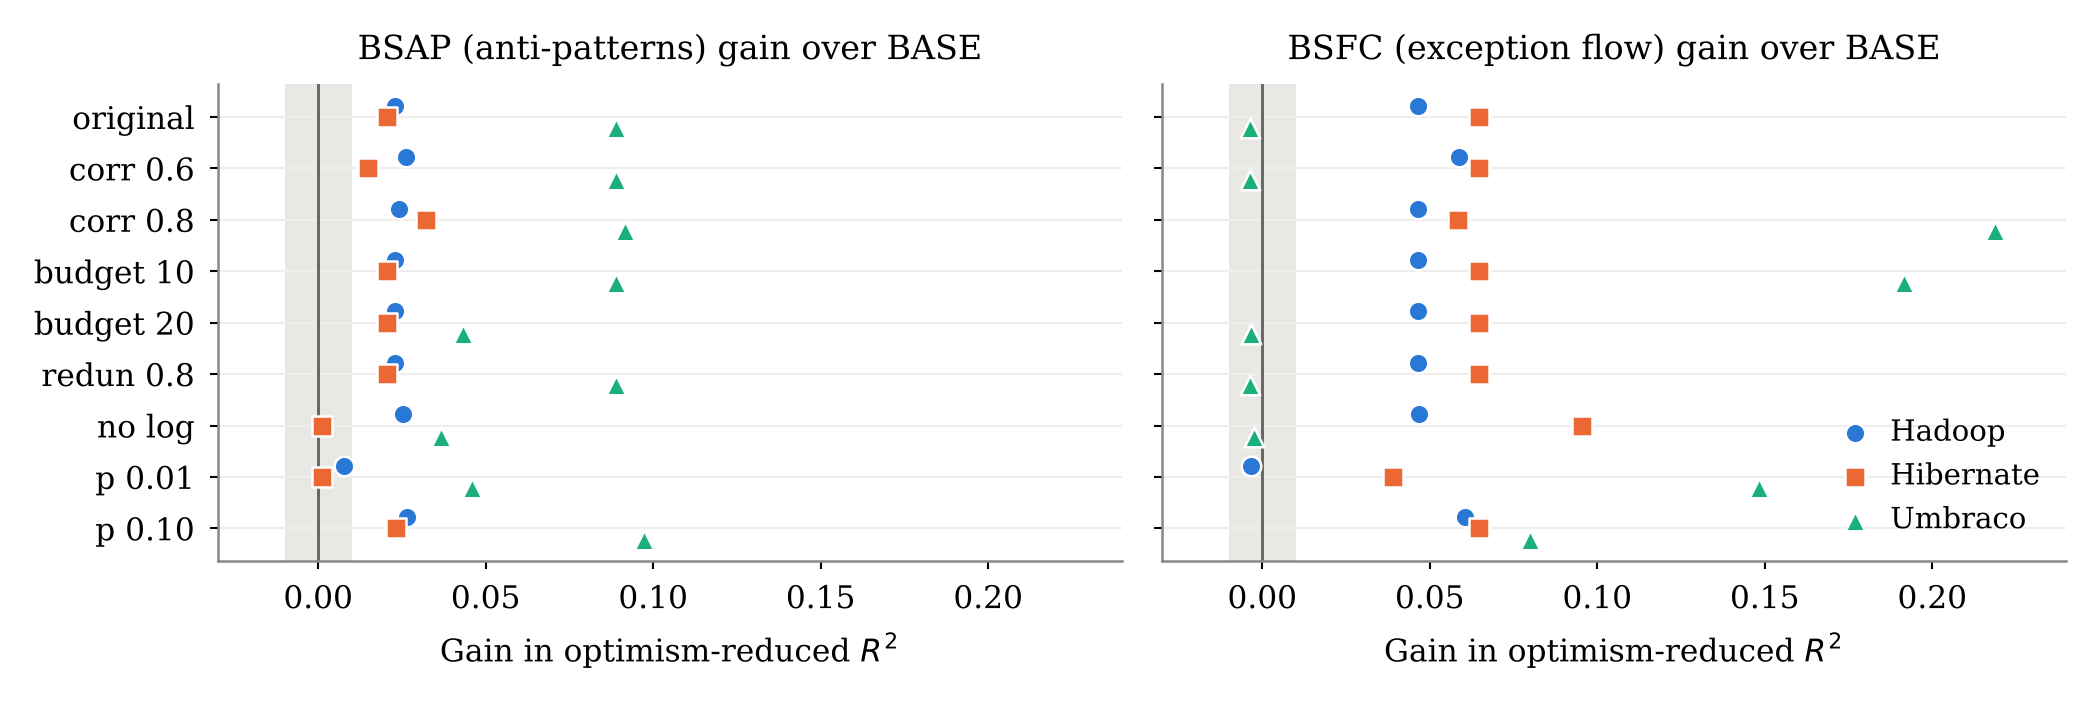
\includegraphics[width=\textwidth]{fig_gain.png}
\caption{Gain in optimism-reduced $R^2$ over BASE for each configuration. The shaded band ($|\text{gain}|<0.01$) is within the run-to-run spread we measured across five seeds (standard deviation $\le 0.003$).}
\label{fig:gain}
\end{figure*}

\section{Interpretation and Validity}
\textbf{What the evidence supports.} The paper's main claims survive reasonable changes to its modeling choices: anti-patterns consistently add explanatory power, and most significant exception handling metrics stay significant with the same sign. The strongest individual claims are the three robust metrics. The evidence does \emph{not} support the paper's negative result for Umbraco's flow metrics. That result depends on the predictor budget forcing the correlation cutoff down to 0.24, which removes most flow metrics before modeling. The authors themselves suspected this; our budget and cutoff variations confirm it.

\textbf{Unexpected results.} Two results need explaining. First, $p<0.01$ removes most findings. That is expected: a stricter threshold drops borderline predictors, so losing a finding there means weaker evidence, not a wrong sign. No finding ever flips sign in any configuration. Second, Umbraco's BSFC $R^2$ moves between 0.08 and 0.30 across configurations, more than any other model. With 230 files, a 15-predictor budget and 23 candidate flow metrics, small changes decide which correlated metrics survive.

\textbf{Strongest threat: selection instability in small samples.} Because significance is read from the model refitted after backward selection, a finding can appear or disappear depending on which correlated metrics happen to survive the reduction steps; this matters most for Umbraco. Two checks are already run: five seeds give identical significant sets (so bootstrap noise is ruled out) and the concept-level score rules out simple average/total swaps. The check still needed is to resample the files themselves and rerun the whole selection pipeline (Section~\ref{sec:next}). A second threat is that we change one setting at a time, which cannot detect interactions such as a lower cutoff combined with a smaller budget.


\section{Remaining Work and Contributions}
\label{sec:next}
\textbf{Artifacts.} The repository now holds the configurable helper functions (\texttt{code/}), the runner and analysis scripts (\texttt{scripts/}), the ten configuration files plus four seed files (\texttt{config/}), each run's raw output (\texttt{output/sensitivity/}), the independent Windows run of the fix (\texttt{output/bsfc\_fix\_run/}), the summary tables behind Tables~\ref{tab:repro}--\ref{tab:stab} and Fig.~\ref{fig:gain} (\texttt{output/summary/}), and an updated README. One configuration runs in about two minutes, so the full set reruns in under half an hour.

\textbf{Scope reductions.} We will not add projects, re-extract metrics, or compare effect sizes across configurations; RQ2 stays at the level of significance and sign. Interactions between settings are limited to the correlation cutoff and the budget, the pair that drives the Umbraco result.

\textbf{Next steps to Milestone 4 (20 November).}
\begin{enumerate}
\item \emph{Selection-stability check (by 13 Nov).} Resample files with replacement 200 times per project, rerun the full pipeline at the original settings, and report how often each of the 15 metrics is selected. This tests the strongest threat directly.
\item \emph{Interaction grid (by 16 Nov).} Run correlation cutoff $\{0.6, 0.7, 0.8\}$ $\times$ budget $\{10, 15, 20\}$ for all projects, nine runs in total.
\item \emph{Independent rerun (by 18 Nov).} A member who did not build the pipeline reruns it from the README on Windows and must match our outputs.
\item \emph{Final analysis and validation plan (20 Nov).}
\end{enumerate}
\emph{Fallback:} if time runs short after the midterm, the interaction grid is dropped first; the selection-stability check and the independent rerun stay.

\textbf{Member contributions.} Table~\ref{tab:contrib} lists completed work.

\begin{table}[!t]
\centering
\caption{Completed contributions since Milestone 2}
\label{tab:contrib}
\footnotesize
\begin{tabular}{@{}p{0.2\columnwidth}p{0.74\columnwidth}@{}}
\toprule
Member & Completed tasks and artifacts \\
\midrule
E. Adegboye & Linux reproduction of the fixed model against Tables 4 and 5; configurable pipeline and runner; ten sensitivity runs and the seed check; analysis scripts, tables and figure; report \\
B. Emeshili & Found and applied the BSFC fix (line 223) and a fixed seed; seeded rerun on Windows (R 4.6.1) confirming Tables 4 and 5; log entry (PR \#1, commits \texttt{bfb43df}, \texttt{2067220}; \texttt{output/bsfc\_fix\_run/}) \\
M. Spensieri & \todo{Marco: what you completed since A2, with the file or commit} \\
\bottomrule
\end{tabular}
\end{table}


\begin{thebibliography}{6}
\footnotesize
\bibitem{padua2018msr}
G.~B. de P\'adua and W.~Shang, ``Studying the relationship between exception handling practices and post-release defects,'' in \emph{Proc. 15th Int. Conf. Mining Software Repositories (MSR)}, 2018, doi: 10.1145/3196398.3196435.
\bibitem{jiarpakdee2021tse}
J.~Jiarpakdee, C.~Tantithamthavorn, and A.~E. Hassan, ``The impact of correlated metrics on the interpretation of defect models,'' \emph{IEEE Trans. Softw. Eng.}, vol.~47, no.~2, pp. 320--331, 2021.
\bibitem{shepperd2014bias}
M.~Shepperd, D.~Bowes, and T.~Hall, ``Researcher bias: The use of machine learning in software defect prediction,'' \emph{IEEE Trans. Softw. Eng.}, vol.~40, no.~6, pp. 603--616, 2014.
\bibitem{tantithamthavorn2017tse}
C.~Tantithamthavorn, S.~McIntosh, A.~E. Hassan, and K.~Matsumoto, ``An empirical comparison of model validation techniques for defect prediction models,'' \emph{IEEE Trans. Softw. Eng.}, vol.~43, no.~1, pp. 1--18, 2017.
\bibitem{harrell2015rms}
F.~E. Harrell, \emph{Regression Modeling Strategies}, 2nd~ed. Springer, 2015.
\end{thebibliography}

\end{document}
